\documentclass{article}
\usepackage{hyperref}
\usepackage{graphicx} % Required for inserting images
\usepackage{booktabs}
\usepackage{pdfpages}
\usepackage{float}
\title{submission_3}
\author{Caden Roberts}
\date{March 2025}

\begin{document}
\begin{titlepage}
    \centering
    \vfill
    {\Huge \bfseries Project Documentation 3\par}
    \vspace{1.5cm}
    {\Huge
        Akash Srinivasan \par \ \par
        Caden Roberts \par \ \par
        Jhovanny Uribe \par \ \par
        Andy Vo \par \ \par
        Ethan Cesario \par \ \par
        Aliyaa Islam \par \ \par
    }
    \vspace{1cm}
    {\Huge \bfseries Mar 3 2025\par}
    \vspace{1.5cm}
    \href{https://github.com/jhovuribe/Physical-Therapy-Hand-Rehabilitation-Device/}{\Huge \bfseries Github}
\end{titlepage}


\section{Design for Manufacture and Assembly}
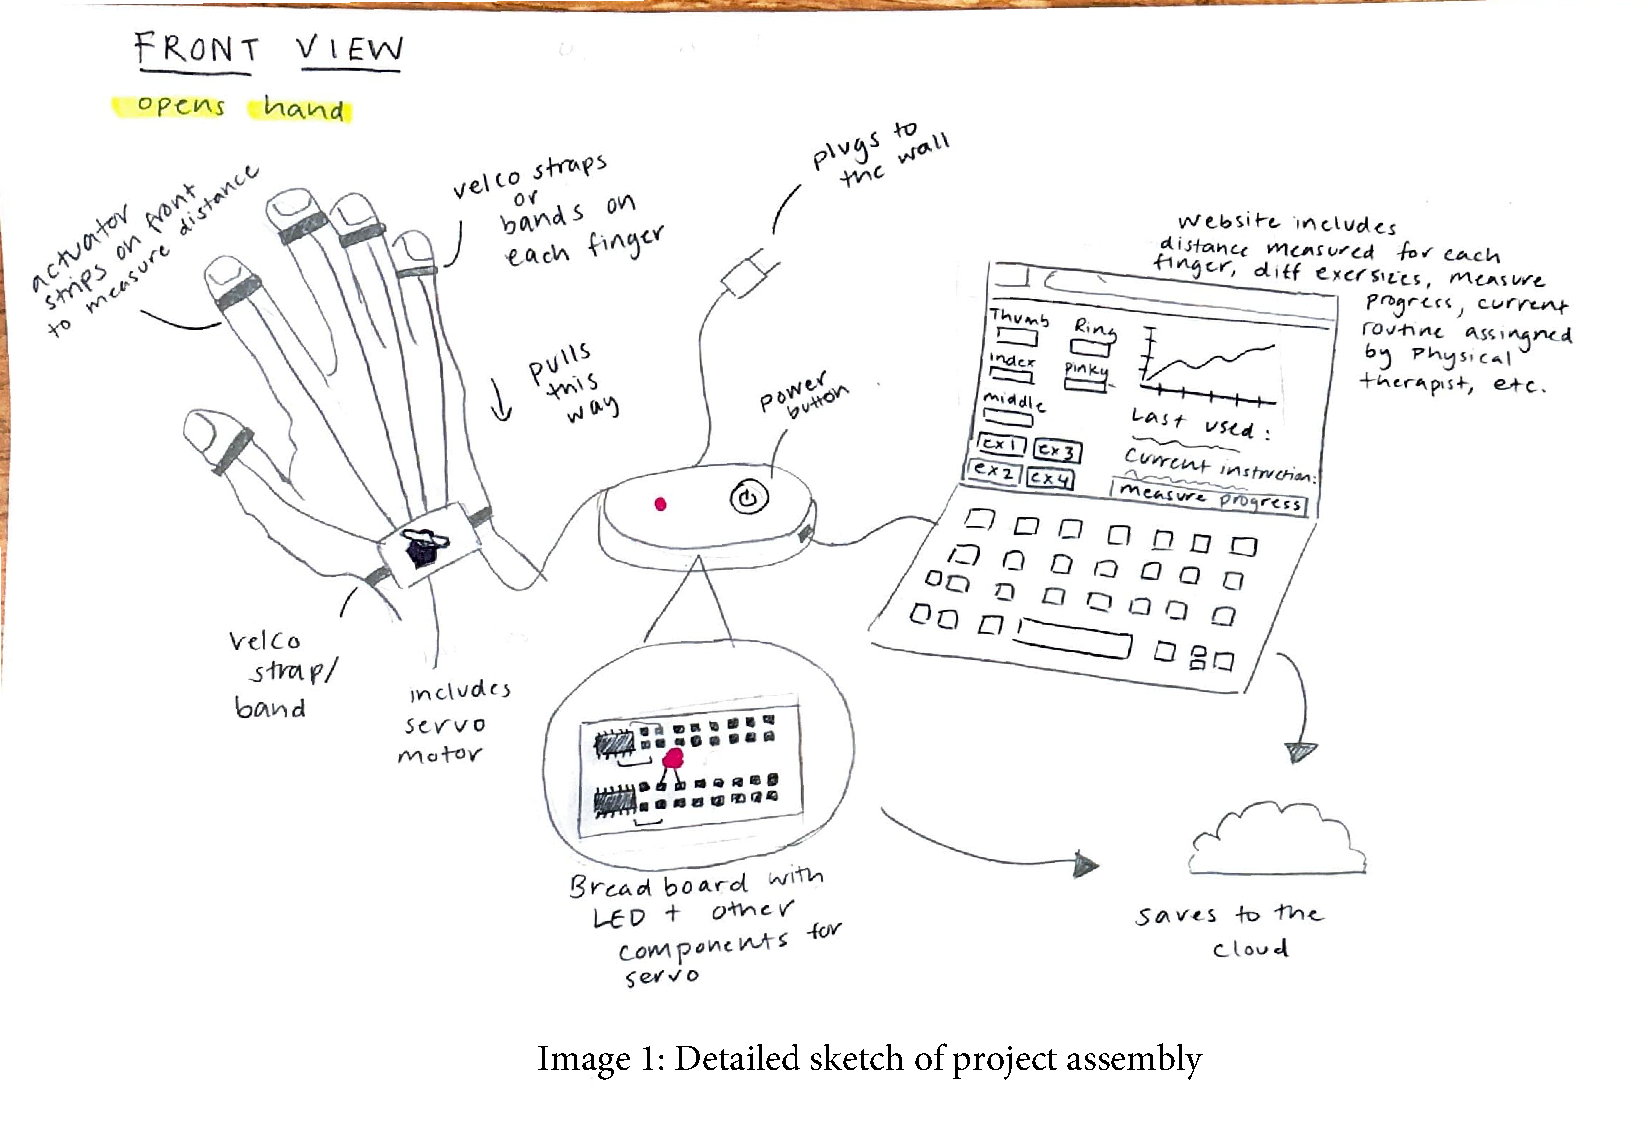
\includepdf[pages=-]{sketch-merged.pdf}
\section{Ethics Statement}
We reference: \href{https://www.apta.org/siteassets/pdfs/policies/codeofethicshods06-20-28-25.pdf}{The Code of Ethics for the Physical Therapist} \\ \\ 
With our physical therapy hand device we aim to address treatment for those who would
benefit from remote commitment to treatment[2][3], adapting to modern trends to benefit
therapists[6] and clients[7] and serving those without consistent access to therapy[8].
\begin{itemize}
\item Principle 2: Physical therapists shall be trustworthy and compassionate in addressing the
rights and needs of patients and clients.
\item Principle 3: Physical therapists shall be accountable for making sound professional judgments.
\item Principle 6: Physical therapists shall enhance their expertise through the lifelong acquisition
and refinement of knowledge, skills, abilities, and professional behaviors.
\item Principle 7: Physical therapists shall promote organizational behaviors and business practices
that benefit patients and clients and society.
\item Principle 8: Physical therapists shall participate in efforts to meet the health needs of people locally, nationally, or globally.
\end{itemize}

\section{Budget for Prototype}

\begin{table}[h]
    \hspace*{-2.2cm}
    \centering
    \begin{tabular}{|l|c|l|c|c|}
        \hline
        \textbf{Item} & \textbf{Quantity} & \textbf{Vendor} & \textbf{Price per Unit (\$)} & \textbf{Total Cost (\$)} \\ 
        \hline
        Flex Sensors & 5 & [Spectra Symbol] & 10.85 & 54.25 \\ 
        \hline
        Microcontroller (ESP32) & 1 & [AITRIP] & 15.99 & 15.99 \\ 
        \hline
        Glove & 1 & [LYDTICK] & 16.99 & 16.99 \\ 
        \hline
        Wiring \& Connectors & 1 (pack) & [Spark Fun] & 5.97 & 5.97 \\ 
        \hline
        Battery Pack & 1 & [Raion Group] & 29.95 & 29.95 \\ 
        \hline
        3D Print Filament & 1 & [AMOLEN] & 29.99 & 29.99 \\ 
        \hline
        Actuator (Micro-Servos) & 1 (10 pack) & [Smraza] & 18.99 & 18.99 \\ 
        \hline
        Server Cost (Monthly) & N/A & [AWS] & Free Tier & Free \\ 
        \hline
        Velcro & 1 & [ULINE] & 20.00 & 20.00 \\ 
        \hline
        \textbf{TOTAL} & & & & \textbf{192.13} \\ 
        \hline
    \end{tabular}
    \label{tab:cost}
\end{table}
\section{Life Cycle Assessment}
\subsection{Goal and Scope Definition}
\subsubsection{Objective}
The LCA aims to assess the environmental footprint of the Thera-Hand rehabilitation device, considering its:
\begin{itemize}
\item Energy consumption (power supply, servos, ESP32).
\item Material usage (PLA, rubber, fishing line, sensors).
\item Manufacturing and transportation impact.
\item End-of-life disposal/recycling feasibility.
\end{itemize}
\subsubsection{Functional Unit}
A single Thera-Hand device is assumed to be used for 2 years before replacement.
\subsubsection{System Boundaries}
This LCA includes:
\begin{itemize}
\item Raw Material Extraction – Plastics, rubber, and electronics production.
\item Manufacturing and Assembly – 3D printing, PCB production, servo motor production.
\item Transportation – From manufacturing to users.
\item Use Phase – Power consumption during operation.
\item End of Life – Disposal, recycling, or potential reuse.
\end{itemize}
\subsection{Inventory Analysis}
\subsubsection{Material Composition and Impact}
\begin{table}[h]
    \hspace*{-3.5cm}
    \centering
    \begin{tabular}{|l|l|l|}
        \hline
        \textbf{Component} & \textbf{Material} & \textbf{Environmental Impact} \\ 
        \hline
        Frame \& Housing & PLA (3D printed) & Low-carbon footprint, biodegradable under specific conditions \\ 
        \hline
        Sensors & Flexible PCB, resistive materials & Electronic waste, difficult to recycle \\ 
        \hline
        Actuators (Servos) & Plastic, copper wiring & High-energy manufacturing, limited recyclability \\ 
        \hline
        Power Supply & Electronic components, metal & Requires responsible e-waste disposal \\ 
        \hline
        Wiring \& Fishing Line & Copper wiring, nylon & Small footprint, but non-biodegradable \\ 
        \hline
    \end{tabular}
    \label{tab:material_composition}
\end{table}
\subsubsection{Energy Consumption(Use Phase)}
Based on prior power consumption estimates:
\begin{table}[h]
    \hspace*{-2.2cm}
    \centering
    \begin{tabular}{|l|c|c|c|}
        \hline
        \textbf{Component} & \textbf{Power Consumption (W)} & \textbf{Usage per day (hours)} & \textbf{Annual Energy (kWh)} \\ 
        \hline
        ESP32 & 1.25W & 2 & 0.91 kWh \\ 
        \hline
        5 SG90 Servos & 6.25W (idle) / 16.25W (peak) & 1 & 5.93 kWh \\ 
        \hline
        Sensors \& LED & 0.15W & 2 & 0.11 kWh \\ 
        \hline
        \textbf{Total Estimate} & $\approx$ 7.65W - 17.65W & - & 6-7 kWh/year \\ 
        \hline
    \end{tabular}
    \caption{Comparison: This is equivalent to a low-power LED bulb running for ~3 months.}
    \label{tab:energy_consumption}
\end{table}
\subsection{Impact Assessment (Environmental)}
\subsubsection{Manufacturing:}
\begin{itemize}
\item Electronics production (ESP32, sensors, servos) has the highest carbon footprint.
\item 3D printing (PLA) requires energy but has a relatively low impact compared to metals.
\end{itemize}
\subsubsection{Use Phase:}
\begin{itemize}
\item Low electricity consumption (~6-7 kWh/year) makes it energy-efficient.
\end{itemize}
\subsubsection{End-of-Life Considerations:}
\begin{itemize}
\item PLA parts are biodegradable in industrial composting but not in landfills.
\item Servos, wiring, and PCBs require responsible e-waste recycling.
\end{itemize}
\subsection{Interpretation and Recommendations}
\subsubsection{Key Findings}
\begin{itemize}
    \item Low Energy Consumption: Thera-Hand is energy-efficient in use.
    \item Minimal Carbon Footprint for PLA: The frame is eco-friendly, but plastics must be disposed
of properly.
    \item E-Waste Challenge: Sensors, servos, and the ESP32 must be recycled properly.
    \item Transportation Impact: If shipped globally, the CO$_2$ footprint increases.
\end{itemize}
\subsubsection{Recommendations}
\begin{itemize}
    \item Optimize 3D Printing Material: Use recycled PLA or biodegradable TPU to reduce waste.
    \item E-Waste Collection Plan: Offer a recycling take-back program for electronics.
    \item Reduce Servo Impact: Use low-power or energy-efficient servos if possible.
    \item Sustainable Packaging: Use biodegradable or recycled materials for packaging.
\end{itemize}

\subsection{Conclusion}
\begin{itemize}
\item Thera-Hand is a low-energy, partially sustainable device.
\item The biggest environmental concern is e-waste disposal of sensors and servos.
\item Efforts to recycle electronic components and use sustainable materials can improve its
eco-friendliness.
\end{itemize}
\section{Test Plan}

\subsection{Ability to be turned on/off}
The device should have the ability to be turned off separately from being unplugged.
\subsubsection{Goal} The Device should be able to be turned on and off while still connected to a direct power source.
\subsubsection{External Factors} Make sure the power connection is stable and not underloaded.
\subsubsection{Equipment} Hand device with external bank, Power Source.
\subsubsection{Steps}
\begin{enumerate}
\item The device should not be connected to any person.
\item The device should be plugged into an AC stable power supply of at least 120V. A
common wall socket is preferred.
\item Load any basic exercise and wait longer than 10 seconds.
\item Turn off the device by pressing the power button on the box connected to the wall. Make
sure to press the power button before the exercise has finished.
\item Observe and measure the time it takes for the device to stop movement.
\item Repeat steps 3-5 multiple times with differing exercises.
\end{enumerate}
\subsection{Ability to download/save metrics}
Data should be stored and sent remotely after each exercise is completed.
\subsubsection{Goal} The Device should be able to remotely send data to an external device that can store
data.
\subsubsection{External Factors} Unstable power supply, unstable internet connection, and connectivity issues.
\subsubsection{Equipment} Hand device with external bank, Power Source, Separate device connected to
internet and connected to device.
\subsubsection{Steps}
\begin{enumerate}
\item Plug the device into a stable 120V AC power supply, preferably a wall outlet.
\item Load the exercise onto the device and begin the workout. Preferably a short workout
routine.
\item Connect the therapist's device to a stable internet connection.
\item Pair the device to a therapist's computer, allowing it to download and store the device's
workout data.
\item Start the workout and wait for it to finish.
\item Observe the download of the device
\end{enumerate}
\subsection{Weight}
Determine the weight of the device that is worn on the hand. Under two pounds.
\subsubsection{Goal} The device should weigh under 2 lbs or 1kg.
\subsubsection{External Factors} The scale should be accurate enough to detect under five pounds and should
be zeroed before use.
\subsubsection{Equipment} Hand device without external bank, small scale.
\subsubsection{Steps}
\begin{enumerate}
\item Unplug the device from the power bank and computer.
\item Place the device on the scale. The glove should be dry and empty. Strings should be attached from servos to fingers.
\end{enumerate}
\subsection{Accuracy of repetition counting}
The device should be tested to report as many repetitions as are being performed. We need to know the degree of error of our data.
\subsubsection{Goal} The device should count the repetitions performed ideally with perfect accuracy.
\subsubsection{External factors} The device should be properly calibrated to recognize when a full range of motion repetition has occurred.
\subsubsection{Equipment} Hand device with external bank, Power Source, Separate device connected to the internet and connected to the device.
\subsubsection{Steps}
\begin{enumerate}
\item Plug the device into a 120V AC outlet.
\item Turn the device on and begin basic squeeze exercises, where fingertips must touch, for 10 seconds.
\item While the device records repetitions, manually count how many repetitions occur until the time is over.
\item Compare the number of repetitions the device reports to the number of repetitions observed.
\end{enumerate}
\subsection{Individual controllability} Each finger should be able to operate independently of any other finger.
\subsubsection{Goal} Verify that each finger is independently programmable and movable.
\subsubsection{External factors} Individual anatomy and flexibility of those being tested.
\subsubsection{Equipment} Hand device with external bank, Power Source, Separate device connected to the internet and connected to the device.
\subsubsection{Steps}
\begin{enumerate}
\item Plug the device into a 120V AC outlet.
\item Turn the device on and verify each finger individually can be pulled in individually.
\item Verify each finger individually can be extended back out.
\end{enumerate}
\subsection{Resting state}
The device should return to a resting state after the completion of each exercise.
\subsubsection{Goal} The device should be verified to return to a neutral state after each exercise is completed.
\subsubsection{External factors} Someone’s anatomy or flexibility may prevent a typical “neutral” resting state.
\subsubsection{Equipment} Hand device with external bank, Power Source, Separate device connected to the internet and connected to the device.
\subsubsection{Steps}
\begin{enumerate}
\item Plug the device into a 120V AC outlet.
\item Turn the device on and begin an exercise.
\item After completion of the exercise, verify that the device has returned to its neutral resting state.
\end{enumerate}
\subsection{Full Range of Motion on each finger}
The device should be able to move in the full range of
motion for each finger. Determine through flex sensor data in the amount of flexion (degrees).
\subsubsection{Goal} The device should demonstrate flexion within the expected biomechanical range (0-90 for DIP, 0-100 for PIP, 0-90 for MCP, depending on finger). Deviation beyond 2.5\% of standard human range to be flagged for recalibration. If the device does not meet the expected range, adjustments in control algorithms and
mechanical design may be necessary.
\subsubsection{External factors}
Ambient temperature variations, Device vibrations and mechanical inconsistencies, Any potential latency in response times.
\subsubsection{Equipment}
Glove with integrated flex sensors, Voltage divider circuit with known resistor (? ohms), Arduino, Computer for data logging and visualization
\subsubsection{Steps}
\begin{enumerate}
    \item Mount the device securely and ensure proper calibration of flex sensors.
    \item Record natural rest position of each finger.
    \item Actuate each finger from full extension to full flexion.
    \item Record flex sensor data at key points of movement (0, 45, 90, etc.).
    \item Repeat the process for each finger, ensuring consistency.
\end{enumerate}

\subsection{Ability to fit on a common hand}
The device should be able to fit securely and comfortably on common hand sizes, using straps for adjust-ability.
\subsubsection{Goal} The device should securely fit common hand sizes without excessive gaps or pressure
points. The adjustable straps should allow for a customized fit without discomfort. If fit issues arise, modifications to strap length, padding, or buckle placement may be
necessary.
\subsubsection{External factors}
Impact of movement on strap security. Any noticeable discomfort due to prolonged wear.
\subsubsection{Equipment}
Robotic/assistive hand device with straps for adjustability. 3D hand model (male/female). Measuring tools for assessing gaps and pressure points (ruler, measuring tape, etc.). User feedback for qualitative comfortability assessment.
\subsubsection{Steps}
\begin{enumerate}
    \item Prepare the hand models and device with adjustable straps. Ensure straps are at their default adjustment before each trial.
    \item Measure the circumference of each hand model at the middle of the hand and forearm.
    \item Place the device on each hand model and secure it using the straps. Adjust the straps for a snug but comfortable fit.
    \item Record strap tension using measuring tape and pressure sensors.
    \item Conduct subjective assessment for comfort and stability.
\end{enumerate}

\subsection{Durability of the device}
\subsubsection{Goal} The device should maintain functional integrity for at least 100,000 flexion cycles without significant degradation. The structural components should withstand typical impact forces without catastrophic failure. Environmental exposure should not lead to material breakdown or loss of functionality. If durability issues arise, material selection, mechanical design, or protective coatings may need revision.
\subsubsection{External factors}
Effects of prolonged use on mechanical performance. Environmental factors leading to premature material failure.
\subsubsection{Equipment}
Robotic/assistive hand device. Mechanical testing rig for repeated flexion cycles. Load cell sensors to measure stress and strain. Environmental chamber for temperature and humidity variations. Impact testing apparatus for drop and shock resistance.
\subsubsection{Steps}
\begin{enumerate}
    \item Mount the device on a mechanical testing rig.
    \item Calibrate sensors to measure force, stress, and performance degradation.
    \item Record initial material integrity and functionality metrics.
    \item Subject each finger mechanism to repeated flexion cycles (minimum 100,000 cycles).
    \item Monitor for signs of wear, stiffness, or failure.
    \item Drop the device from various heights onto different surfaces. 
    \item Assess structural damage and continued operability.
    \item Expose the device to temperature fluctuations (-10C to 50C) and high humidity.
    \item Evaluate material degradation and operational stability.
\end{enumerate}

\begin{table}[H]
    \hspace*{-1cm}
    \centering
    \begin{tabular}{|c|c|}
        \hline
        \textbf{Name(s)} & \textbf{Date and Location} \\
        \hline
        \ & \ \\
        \hline
        \textbf{Test 1:} Did the power turn off? (Yes/No) & \\
        \hline
        \textbf{Test 2:} Was data remotely sent? (Yes/No) & \\
        \hline
        \textbf{Test 3:} Weight: (kg/lbs) & \\ 
        \hline
        \textbf{Test 4:} What accuracy were the repetitions counted to? (\%) & \\
        \hline
        \textbf{Test 5:} How many fingers were individually controllable? (0-5) & \\
        \hline
        \textbf{Test 6:} Did the device return to a resting state? (Yes/No) & \\
        \hline
        \textbf{Test 7:} Full Range of Motion on each finger? (Yes/No) & \\
        \hline
        \textbf{Test 8:} Ability to fit on
        common hand? (Yes/No) & \\
        \hline
        \textbf{Test 9:} Device
        Durability acceptable? (Yes/No) & \\
        \hline
    \end{tabular}
    \caption{Test Log}
    \label{tab:test_log}
\end{table}

\section{Updates}
\subsection{Need Statement}
Physical therapy for hand rehabilitation is a time- and cost-intensive process with limited at-home alternative options; providing an easy-to-produce and cheap-to-manufacture device
\subsection{Goal Statement}
We aim to reduce physical therapy visits by up to 50\%, subsequently reducing insurance costs by designing a cost-effective device.
\subsection{Design Objective}
Design a cost-effective solution that is user-friendly and streamlines the rehabilitation process.
\subsection{Morphological Chart}
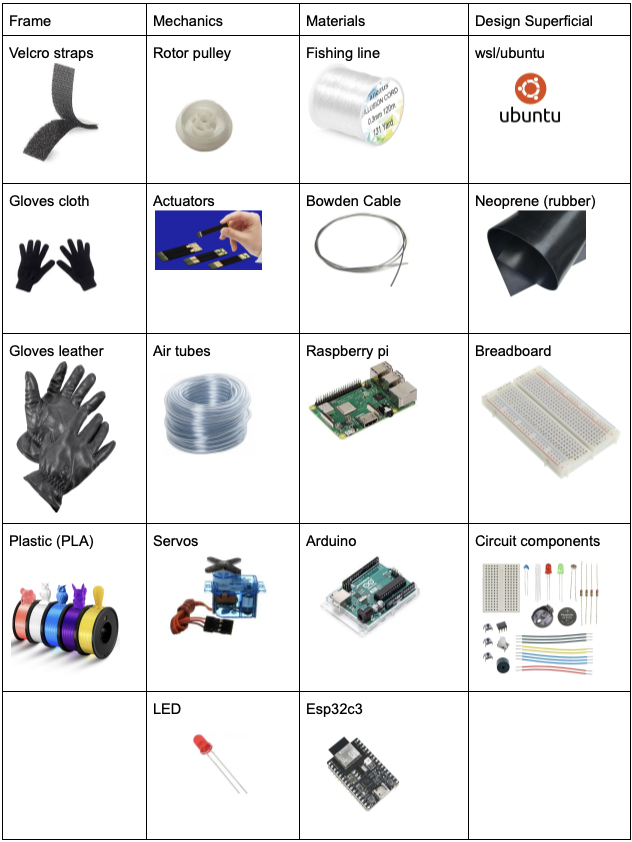
\includegraphics[width=12cm]{morpho.png}
\subsection{Gantt Chart}
\href{https://docs.google.com/spreadsheets/d/12JjnpXyDDq8c87AdqVN5jQ46xVcHvgcuxsZTP0hWSw0/edit?usp=sharing}{Link to Updated Gantt Chart}
\newline
\newline
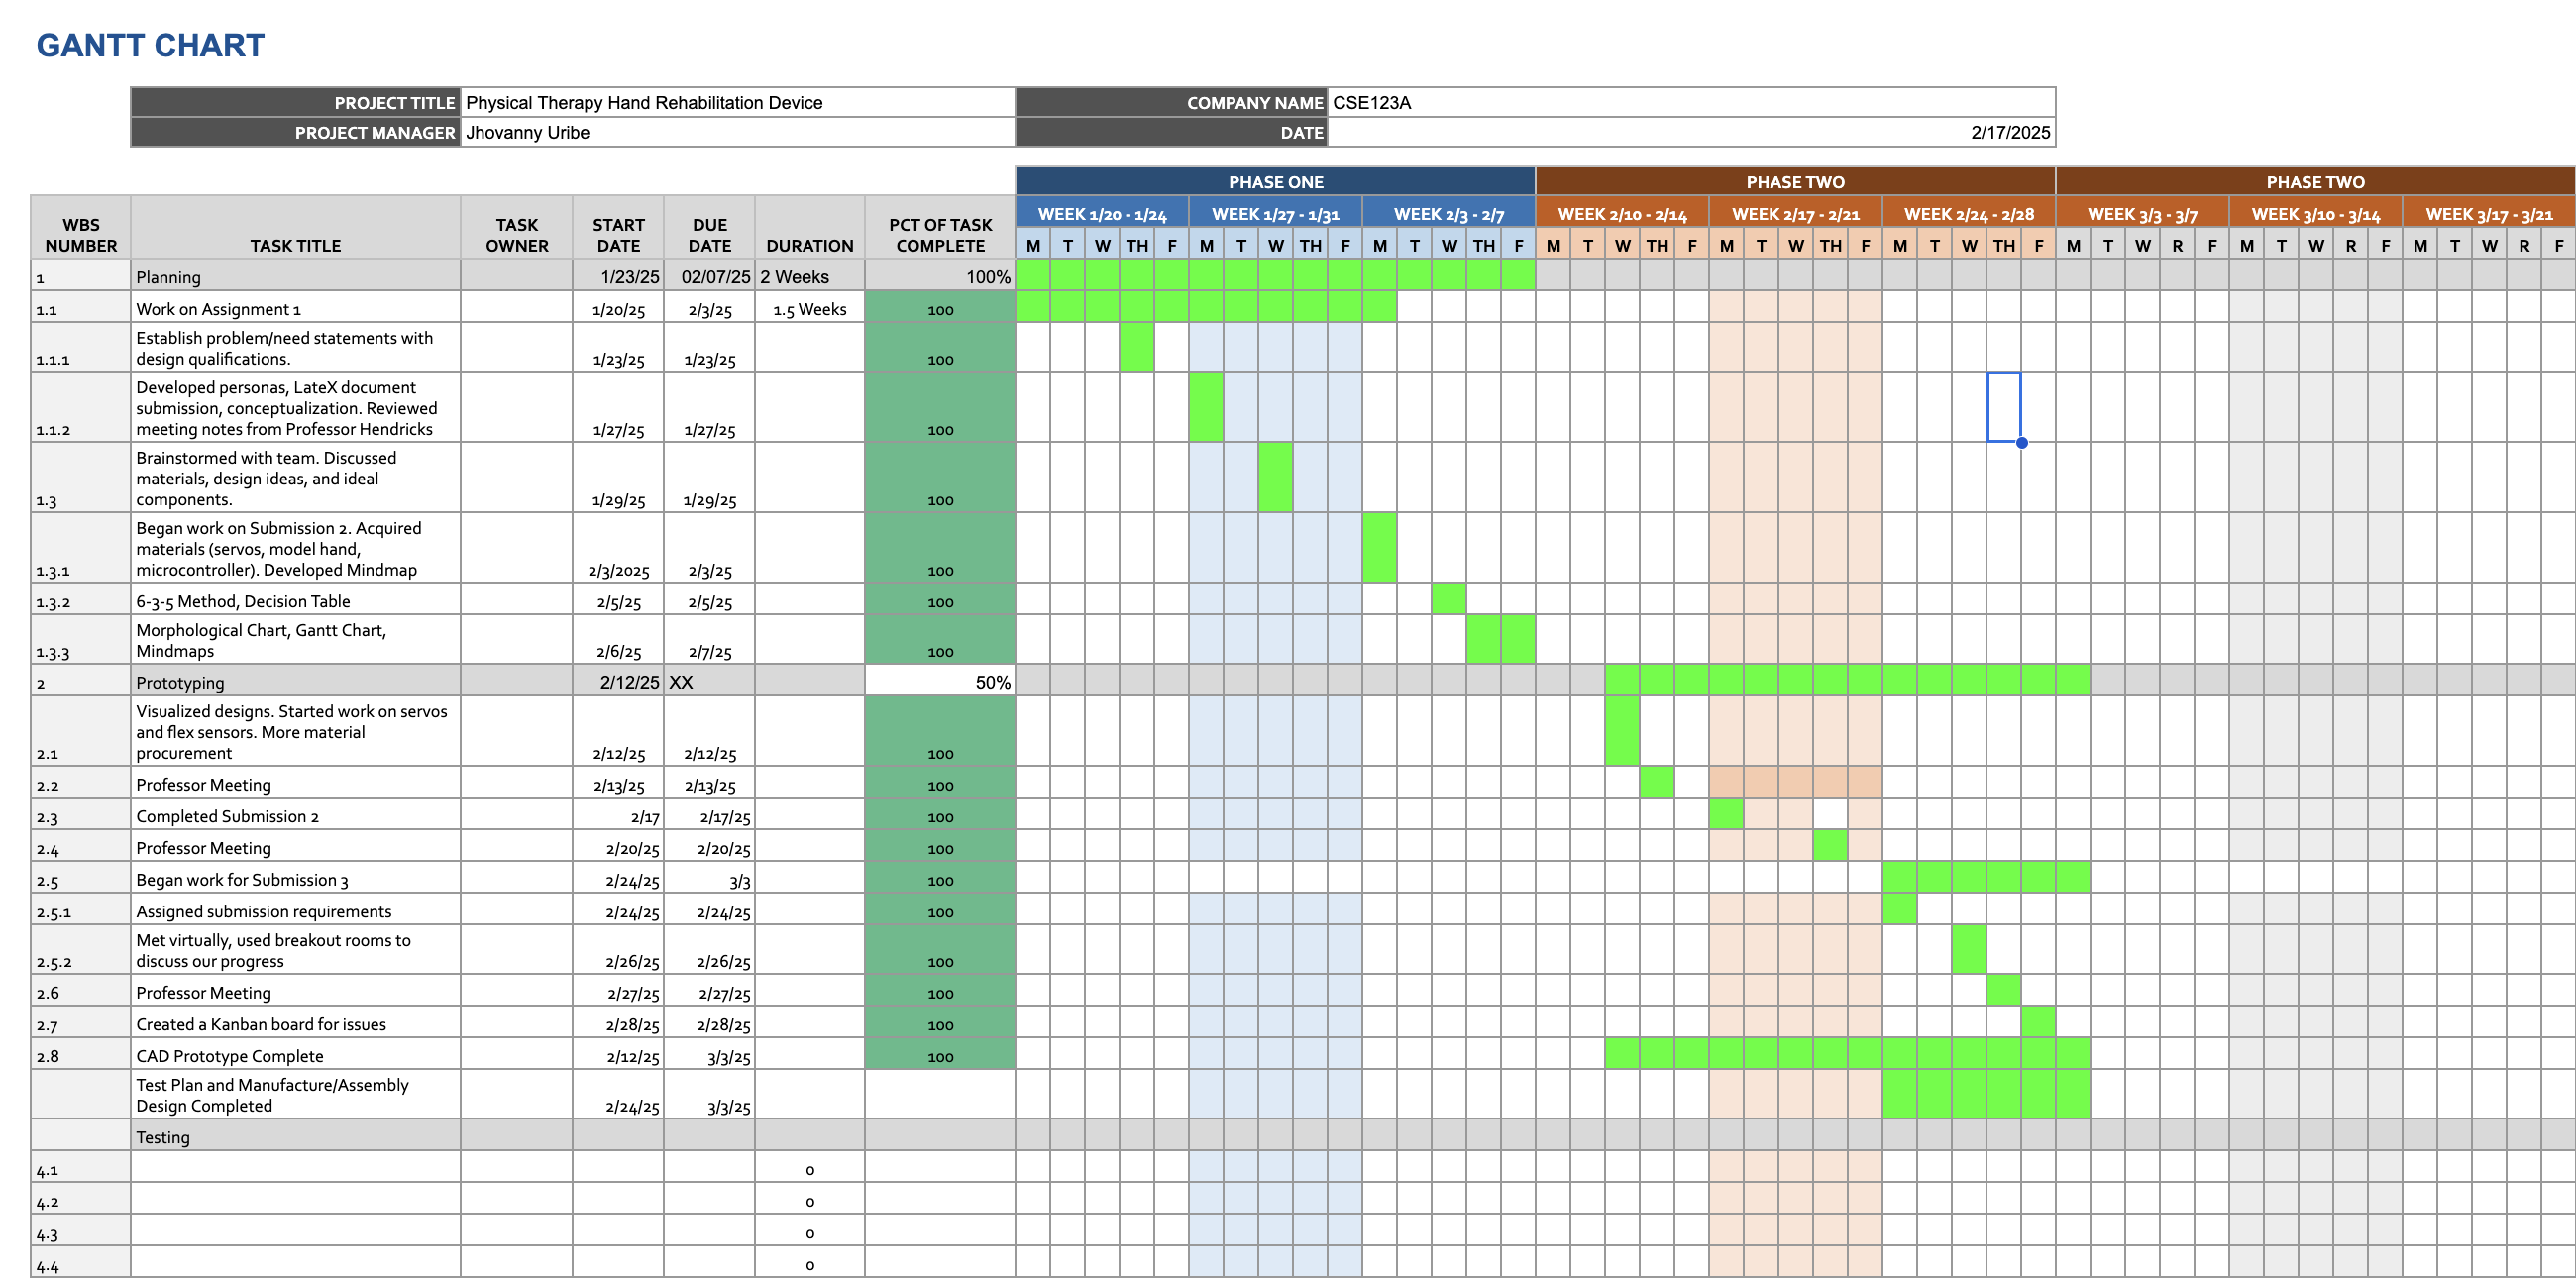
\includegraphics[width=1.5\textwidth]{Gantt Chart pic.png}
\end{document}
